
\section{Non-inverting buck-boost converter\label{N_INV_BB}}
		
The Non-inverting Buck-Boost converter is a DC to DC converter that allows the voltage at its output to be higher or lower than the voltage at its input. The topology can be seen in figure \ref{N_INV_BB_SCHEMATIC}. It uses 4 switches, of which 2 are controlled devices. 
		

\begin{figure}[htbp]
	\begin{center}
	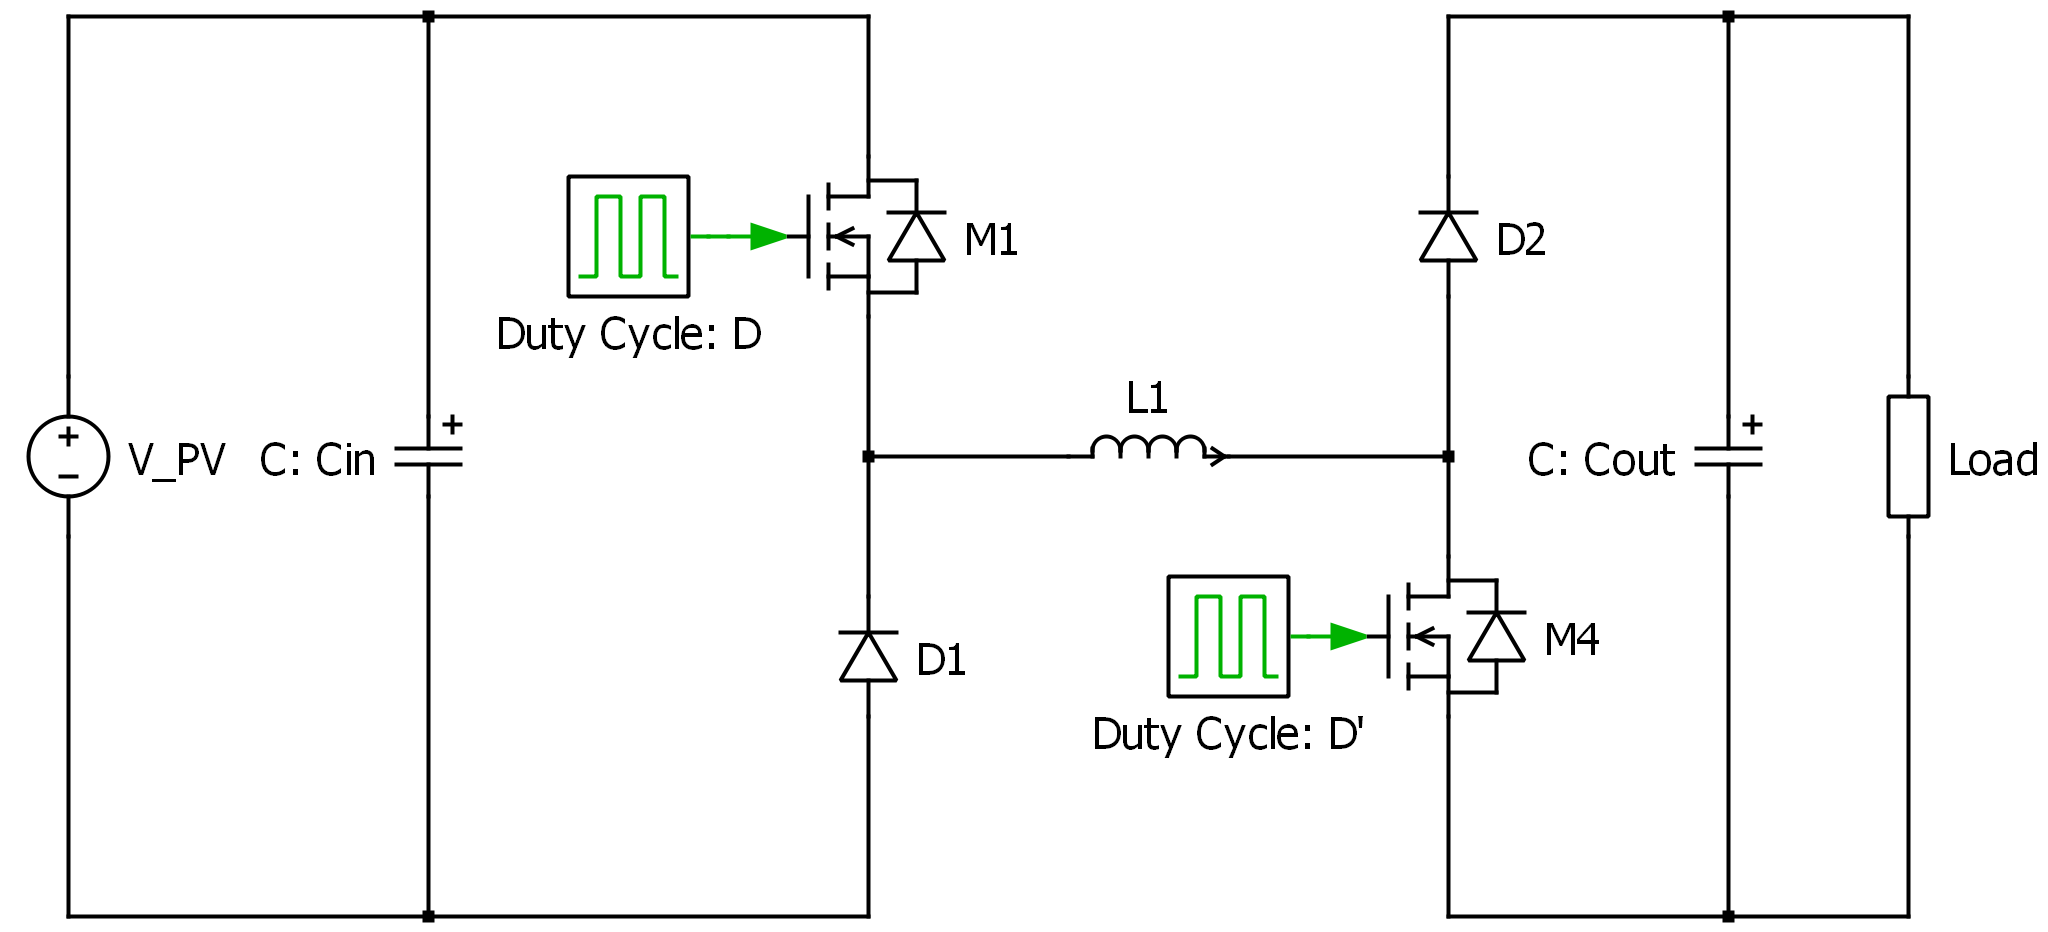
\includegraphics[width=0.7\textwidth]{../Pictures/2_d_H_B_BB}
	\caption{Non-inverting buck-boost converter.}
	\label{N_INV_BB_SCHEMATIC}
	\end{center}	
\end{figure}

		
The controller can force the system to work in any of the following modes:

\begin{enumerate}
	\item Buck $\rightarrow$ $ D \subset [0,1];	 D' = 0 $
	\item Boost $\rightarrow$ $ D = 1;	 D' \subset [0,1] $
	\item Buck-Boost $\rightarrow$ $ D \subset [0,1]; D' \subset [0,1] $
\end{enumerate}

One of the main drawbacks of the topology is the control's complexity, which must calculate the appropriate duty cycle $D$ and $D'$ in any of the modes and also the transition between these modes. 
		
Usually the inverter's input voltage is fixed to some value higher than the grid's voltage. The possibility of higher and lower voltages at the converter's output allows different ways of associating photovoltaic modules. Then the user is able to arbitrarily decide how many PV modules to link in series. Differently of what would happen in the case of Buck or Boost converters where the constraints regarding the number of panels are tighter.
		
Compared with other topologies that can have both higher and lower voltages at the output, such as the SEPIC or ZETA converters, this converter features a single inductor and no intermediate capacitor. With such reduction in passive components the price, efficiency and power density rises significantly [Under the hood of a noninverting buck-boost converter]. 
		
Although this topology exhibits appropriate features, it can be further improved by replacing the diodes by MOSFETs. The circuit may be seen in figure \ref{BID_N_INV_BB_SCHEMATIC}, it's called Bidirectional Non-Inverting Buck-Boost converter. With this variation, the following changes occur:
		
\begin{enumerate}
	\item The system becomes bidirectional.
	\item The conduction losses are decreased. \textbf{--> Discuss with supervisor}
\end{enumerate}
	
If the system is bidirectional it can be used in different MIC strategies, such as \textbf{ ++reference to the introduction figure with the MICs outputting power to the PV++}. Or even implement diagnosis features with the panels' electroluminescence, whenever these are fed enough power. 
		
		
As seen in figure \ref{BID_N_INV_BB_SCHEMATIC}, notice that duty cycles of the switches that replace the diodes are $\overline{D}$ and $\overline{D'}$.
		
The main drawback is the increased difficulty of the driver circuitry. And the requirement of a dead time in order to avoid the short circuit of $FET_1$ and $FET_3$ or $FET_2$ and $FET_4$ which could damage the system. When using diodes, the system is intrinsically protected against a shoot-through event. 	
		
\begin{figure}[htbp]
	\begin{center}
	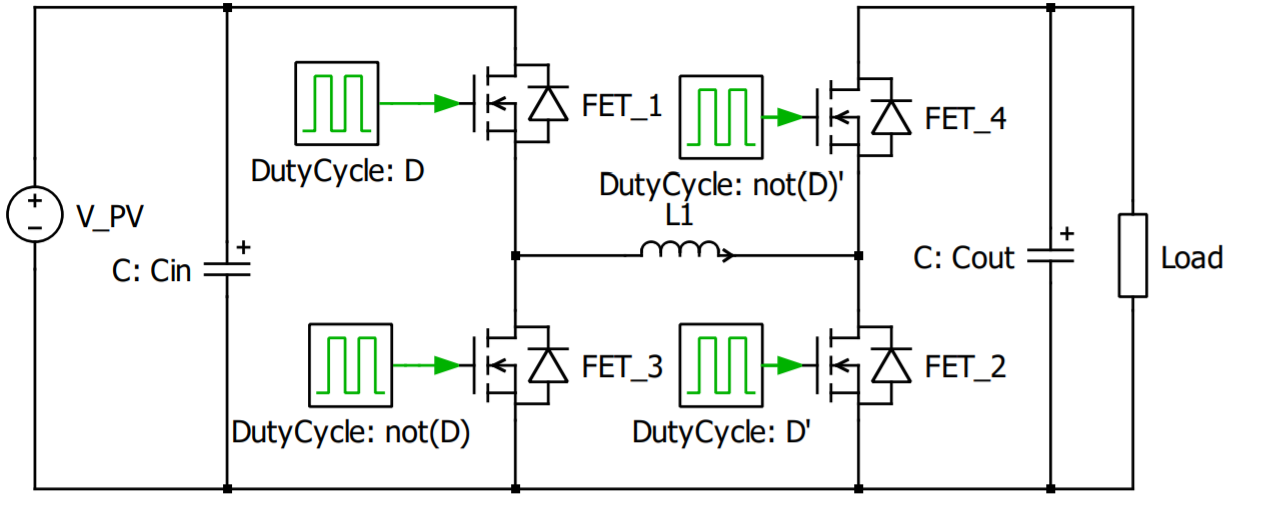
\includegraphics[width=0.7\textwidth]{../Pictures/BID_H_B_BB}
	\caption{Bidirectional Non-inverting buck-boost converter.}
	\label{BID_N_INV_BB_SCHEMATIC}
	\end{center}
\end{figure}



